\section*{Progress Report}
\subsection{What has been accomplished to date}

Following the schedule in our proposal, we have downloaded the Yelp dataset\footnote{http://www.yelp.com/dataset\_challenge} and preprocessed the data. We start from exploiting the basic business information, parsed as below:\\
\emph{
\small
\indent name: Forever 21\\
\indent id: 7lbvsGKzhjuX3oJtaXJvOg\\
\indent longitude: -111.964485\\
\indent latitude: 33.383123\\
\indent stars: 3.5\\
\indent categories: Women's Clothing,Men's Clothing,Fashion,Shopping,Accessories
}

To implement $k$-NN algorithm, we first need to define the neighbors of each business. As we can notice, a food plaza should encompass a diversity of popular restaurants, a shopping mall always includes many brand stores, and a bar street is occupied by various lively pubs. Following the homophily principle in the same category, we intuitively give the definition of business neighbor.

\begin{defn}[Business Neighbor]
Business A is the neighbor of business B, iff $category_A \cap category_B \neq \varnothing$.
\end{defn}

In this way, the popularity (stars) of a certain business can be inferred by its neighbor in the same category. This is exactly the idea of $k$-NN algorithm. We implemented a 10-fold cross-validation. Specifically, in each round, we take one fold as test set and the remaining nine folds as training set. For each business in the test set, the average star rating of its $k$ nearest neighbors would be its predicted rating. For evaluation, mean squared error (MSE) is used to quantify the difference between predicted values $\hat{Y}_i$ and the ground truth $Y_i$.

$$MSE=\frac{1}{n}\sum_{i=1}^{n}(\hat{Y}_i-Y_i)^2$$

<<<<<<< HEAD
In the experiments, we set $k=1,\cdots,9$ respectively. As we can see the experimental result in Figure~\ref{knn}, the larger $k$ is, the better MSE we can achieve. Notice that $Y_i$ ranges from 1 to 5. This result leads us to a doubt that whether exploiting the geographical neighbors for a business with the same category is really a valid approach to determine its popularity. It is likely that a more sophisticated method would be necessary.

\begin{figure*}[t]
\centering
    \begin{minipage}[l]{\columnwidth}
      \centering
      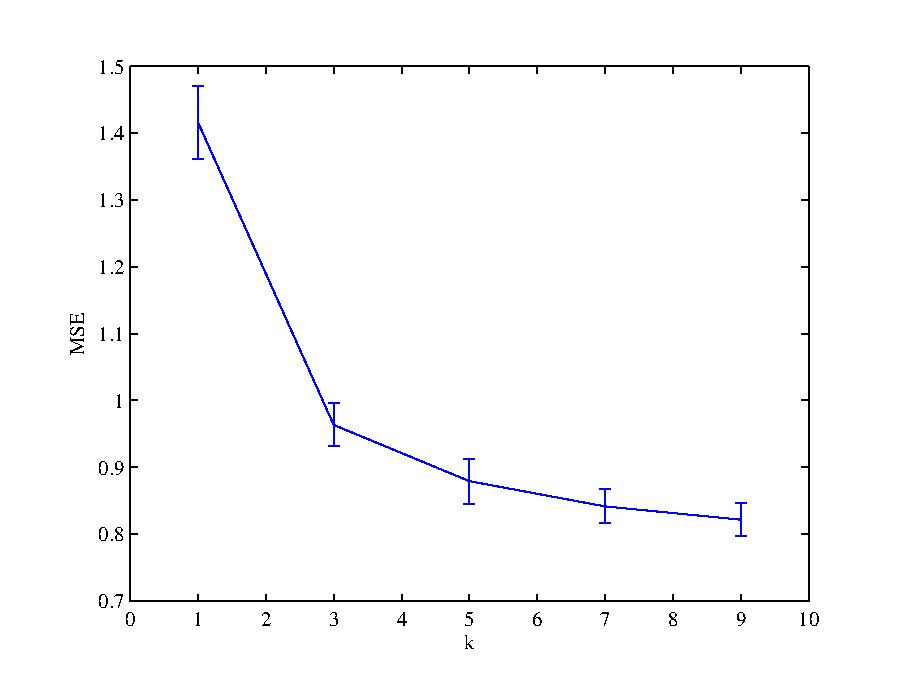
\includegraphics[width=1\textwidth]{knn}
    \end{minipage}
  \caption{Performance of k-NN algorithm (mean $\pm$ std).}\label{knn}
\end{figure*}

\subsection{What remains to be done}

The next step for us is to consider how to exploit the correlations between different types of businesses. In the $k$-NN baseline, the problem is simply decomposed into independent subproblems for each category, where only the homophily principle is leveraged. However, there might be counteractions between certain pairs of businesses. An interesting idea is to propagate such information, either positive or negative, across different types of businesses within the neighborhood. An alternative approach is to extract some informative features from the dataset to facilitate the prediction task.
=======
In the experiments, we set $k$ to $5$. The final experimental result is $0.879 \pm 0.034$ (mean $\pm$ std).
Notice that $Y_i$ range from 1 to 5.

\subsection{What remains to be done}

The next step for us is to consider how to exploit the correlations between different types of businesses. In the $k$-NN baseline, the problem is simply decomposed into independent subproblems for each category, where only the homophily principle is leveraged. However, there might be counteractions between certain pairs of businesses. An interesting idea is to propagate such information, either positive or negative, across different types of businesses within the neighborhood. An alternative approach is to extract some informative features from the dataset to facilitate the prediction task. 
>>>>>>> 70fbd973b171cd91059a02b10952772e96f1b12e
